\documentclass{article}
\usepackage[utf8]{inputenc}
\usepackage{hyperref}

\title{Baloiço}

\author{Alexandre Barbosa e Miguel Roldão \\
\\\href{mailto:alexandre.barbosa@tecnico.ulisboa.pt}{alexandre.barbosa@tecnico.ulisboa.pt} 
\\
\href{mailto:miguel.roldao@tecnico.ulisboa.pt}{miguel.roldao@tecnico.ulisboa.pt} 
   }
\date{Janeiro de 2019}

\usepackage{natbib}
\usepackage{graphicx}
\usepackage[portuguese]{babel}
\usepackage{titlesec}
\setcounter{secnumdepth}{3}
\usepackage{textalpha}

\begin{document}

\maketitle

\section{Introdução}
     O movimento de uma criança sentada num baloiço pode ser modelado como o de um haltere composto por três massas. A equação de movimento para este sistema, quando são feitas aproximações razoáveis para a amplitude, é a de um oscilador harmónico forçado \citep{swing}.\\\\
     O presente projeto é um programa, desenvolvido na linguagem C com o '\textit{toolkit}' GTK 3+ \citep{gtk3}, que simula e representa graficamente este movimento, permitindo alterar os seus parâmetros em tempo real, bem como visualizar os gráficos que relacionam as grandezas físicas que o descrevem \citep{tf}.

\begin{figure}[ht]
\centering
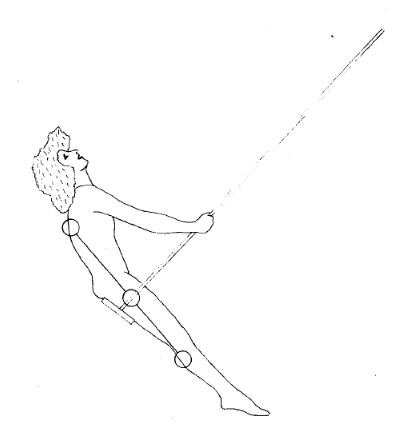
\includegraphics[scale=0.45]{swing_seated.png}
\caption{ A relação entre uma criança num baloiço e o modelo utilizado \citep{swing}}
\end{figure}

\section{Manual do Programa}

Ao iniciar o programa, é aberta uma janela que se ajusta automaticamente às dimensões do ecrã, na qual é possível visualizar a simulação, os gráficos e alterar os seus parâmetros. Ao utilizador, na área de desenho da simulação, é mostrado um \hyperlink{figure2}{esquema} que ilustra as posições das massas, fios, eixos e ângulos.

\begin{figure}[ht]
\centering
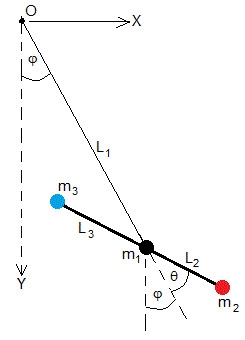
\includegraphics[scale=0.6]{swing_start.jpg}
\caption{\hypertarget{figure2}{Esquema do Modelo} \citep{columpio}}
\end{figure}

\subsection{Painel de Controlo}

O Painel de Controlo contém diversas '\textit{widgets}' que alteram, com base no '\textit{input}' do utilizador, os parâmetros de execução do programa, em tempo real.

\subsubsection{'\textit{Slider Scales}' (Barras Deslizantes)}

As '\textit{slider scales}' (barras deslizantes) permitem alterar parâmetros quando o utilizador move o cursor. Uma '\textit{label}' identifica a grandeza a ser alterada e mostra o seu valor atual. As '\textit{scales}' alteram o valor das massas (m\textsubscript{1}, m\textsubscript{2}, m\textsubscript{3}), o comprimento dos fios (l\textsubscript{1}, l\textsubscript{2} e l\textsubscript{3}), a frequência angular (\omega$), a aceleração da gravidade (\textit{g}) e o fluxo do tempo.

\subsubsection{'\textit{Combo Boxes}' (Caixas de Combinação)}

As  '\textit{combo boxes}' (caixas de combinação) dão a possibilidade de escolher parâmetros predefinidos, alterando simultaneamente os valores de várias  '\textit{scales}'. A primeira  '\textit{combo box}' permite escolher se se trata de uma criança ou de um adulto e a segunda o planeta (do sistema solar) em que decorre a simulação.

\subsubsection{\textit{Botões de ''Restart'' e ''Play'}' (Reiniciar e Começar)}

Os botões de "Restart" e "Play", ao serem pressionados, recomeçam e param ou continuam a simulação, respetivamente. 

\subsection{Condições Iniciais}

O painel das Condições Iniciais contém as '\textit{widgets}' que alteram as condições iniciais da simulação. Ao alterar o valor das '\textit{scales}', a simulação recomeça.

\subsubsection{'\textit{Slider Scales}' (Barras Deslizantes)}

As '\textit{slider scales}' (barras deslizantes) desta secção alteram os valores dos ângulos iniciais (\theta\textsubscript{0}$ e   \phi\textsubscript{0}$) e da velocidade angular inicial em \phi$.

\subsubsection{Cores}

Um '\textit{radio button}' (botão de rádio) permite escolher a massa cuja cor é alterada. Ao pressionar o botão "Cor", é aberta uma janela ('\textit{dialog box}') na qual é possível selecionar a nova cor (o que não reinicia a simulação).

\subsection{Gráficos}

O painel dos Gráficos contém as '\textit{widgets}' que controlam, em tempo real, com base nas escolhas do utilizador, as suas definições.

\subsubsection{'\textit{Combo Boxes}' (Caixas de Combinação)}

As  '\textit{combo boxes}' (caixas de combinação) permitem escolher quais os gráficos a mostrar. Uma '\textit{label}' identifica a qual dos gráficos esta a '\textit{combo box}' se refere.

\subsubsection{Cores}
Ao pressionar o botão "Cor", é aberta '\textit{dialog box}' na qual é possível selecionar a cor dos gráficos. Uma '\textit{label}' identifica a qual dos gráficos o botão se refere.

\subsubsection{'\textit{Check Box}' (Caixa de Seleção)}

A '\textit{check box}' "Mostrar Valores"  permite escolher se os valores dos gráficos desenhados são impressos ou não no canto superior esquerdo do ecrã.

\subsubsection{'\textit{Slider Scales}' (Barras Deslizantes)}

As \textit{slider scales} neste painel permitem ajustar a escala vertical ou a escala do tempo (horizontal), de ambos os gráficos, simultaneamente.

\subsubsection{Apagar Gráficos}

Ao ser pressionado, este botão apaga os gráficos desenhados.

\bibliographystyle{plain}
\bibliography{references.bib}

\end{document}
